\newpage
\section{Data Model and Description}
\quad There are four main data classes which are Event, User and Weather classes.
\begin{figure}[tbh]
  \begin{center}
  % Requires \usepackage{graphicx}
  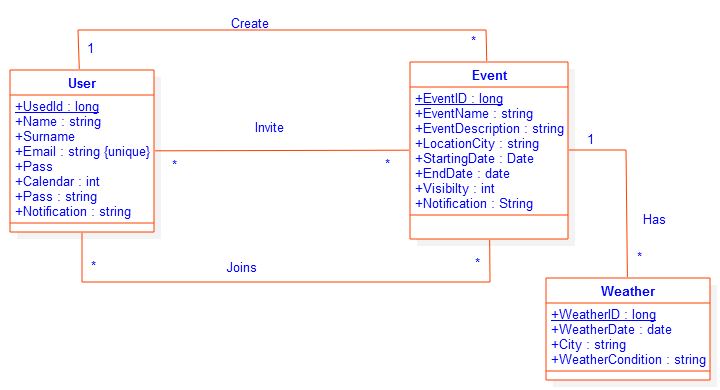
\includegraphics[width=150mm]{ClassDiagram}
  \caption{Class Diagram}\label{Fig :}
  \end{center}
\end{figure}

\subsection{User}
\quad User class stores user details, calendar visibility and notifications received.
\begin{figure}[tbh]
  \begin{center}
  % Requires \usepackage{graphicx}
  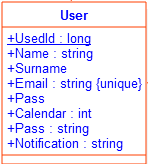
\includegraphics[width=50mm]{UserClassDiagram}
  \caption{User Class Diagram}\label{Fig :}
  \end{center}
\end{figure}

\subsection{Event}
\quad This class stores the event details, event visibility and the notifications for this event to its participant users. There are three different relations between this class and the User class. Two Many to many relation called invite and joins and one one to many relation called create.
\begin{figure}[tbh]
  \begin{center}
  % Requires \usepackage{graphicx}
  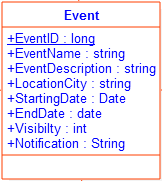
\includegraphics[width=50mm]{EventClassDiagram}
  \caption{Event Class Diagram}\label{Fig :}
  \end{center}
\end{figure}

\subsection{Weather}
\quad This class stores the weather information for events. Every event has at least one weather information so, there is a one to many relation.
\begin{figure}[tbh]
  \begin{center}
  % Requires \usepackage{graphicx}
  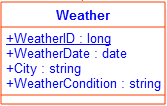
\includegraphics[width=50mm]{WeatherClassDiagram}
  \caption{Weather Class Diagram}\label{Fig :}
  \end{center}
\end{figure}
